% Intended LaTeX compiler: pdflatex
\documentclass[../main]{subfiles}

\use{upgreek}
\def\tau{\uptau}


\begin{document}

\section{Teorema di Escissione}
\label{sec:org7abe800}
Sia \(R\) un \href{20241219112842-pid.org}{PID}.
\begin{thm}
Sia \((X,A)\) una \href{20250122154728-coppia_topologica.org}{coppia topologica} e sia \(U \subseteq A\) un \href{20250103145124-topologia.org}{aperto} di \(X\) tale che la \href{20250103144944-chiusura_topologica.org}{chiusura} \(\operatorname{cl}_{X}(U) \subseteq \mathring{A}\).
Allora i \href{20241205141053-r_moduli.org}{moduli} di \href{20250120164857-modulo_di_omologia_dei_complessi_di_catene.org}{omologia} \href{20250122154903-omologia_singolare_relativa.org}{singolare relativa} sono \href{20241206115416-morfismi_r_moduli.org}{isomorfi}:
\begin{equation*}
	H_{q}(X\setminus U, A\setminus U) \cong H_{q}(X,A).
\end{equation*}
Isomorfismo è la mappa indotta da \(i:(X\setminus U, A\setminus U)\hookrightarrow (X,A)\) tramite il \href{20241205131958-funtore.org}{funtore} \href{20250126191208-funtore_da_topp_a_rmod_di_omologia.org}{di omologia}.
\end{thm}
\begin{thm}
Sia \(X\) uno spazio topologico e siano \(X_{1},X_{2} \subseteq X\) tali che l'\href{20250131155822-operazioni_insiemistiche_tra_classi_mk.org}{unione} delle \href{20250122181431-parte_interna.org}{parti interne} dia tutto lo spazio: \(X=\mathring{X}_{1}\cup \mathring{X}_{2}\).
Allora i \href{20241205141053-r_moduli.org}{moduli} di \href{20250120164857-modulo_di_omologia_dei_complessi_di_catene.org}{omologia} \href{20250122154903-omologia_singolare_relativa.org}{singolare relativa} sono \href{20241206115416-morfismi_r_moduli.org}{isomorfi}:
\begin{equation*}
	H_{q}(X_{1}, X_{1}\cap X_{2}) \cong H_{q}(X,X_{2}).
\end{equation*}
Isomorfismo è la mappa indotta da \(i:(X_{1},X_{1}\cap X_{2})\hookrightarrow (X,X_{2})\) tramite il \href{20241205131958-funtore.org}{funtore} \href{20250126191208-funtore_da_topp_a_rmod_di_omologia.org}{di omologia}.
\label{thm:ESCPRIMO}
\end{thm}
\begin{oss}
I teoremi sono equivalenti. Questo è chiaro considerando la Figura~\ref{fig:eqescescprimo} e ponendo
\begin{align*}
X\setminus U &\leftrightarrow X_{1}\\
A &\leftrightarrow X_{2}\\
A\setminus U &\leftrightarrow X_{1}\cap X_{2}
\end{align*}
\end{oss}

\begin{figure}
\begin{equation*}
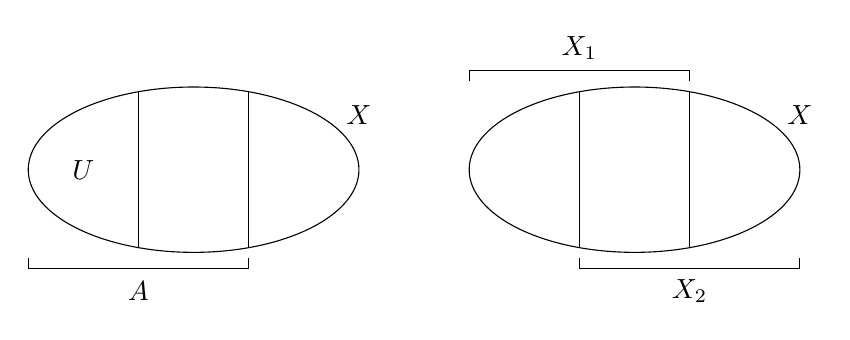
\begin{tikzpicture}[scale=0.7]
% Draw the main ellipse
\draw (0,0) ellipse (3 and 1.5);
\draw (7+1,0) ellipse (3 and 1.5);

% Draw the vertical dividing lines
\draw (-1,-1.41) -- (-1,1.41);
\draw (1,-1.41) -- (1,1.41);
\draw (7+1-1,-1.41) -- (7+1-1,1.41);
\draw (7+1+1,-1.41) -- (7+1+1,1.41);

\node at (3,1) {$X$};
\node at (7+1+3,1) {$X$};
\node at (-2,0) {$U$};
\node at (-1,-2.2) {$A$};
\node at (7+1-1,+2.2) {$X_1$};
\node at (7+1+1,-2.2) {$X_2$};

\draw (-3,-1.6) -- (-3,-1.8) -- (1,-1.8) -- (1,-1.6);
\draw (7+1-3+2,-1.6) -- (7+1-3+2,-1.8) -- (7+1+1+2,-1.8) -- (7+1+1+2,-1.6);
\draw (7+1-3,1.6) -- (7+1-3,1.8) -- (7+1+1,1.8) -- (7+1+1,1.6);
\end{tikzpicture}
\end{equation*}
\caption{\label{fig:eqescescprimo}Equivalenza tra ESC e ESC'}
\end{figure}
\subsection{Dimostrazione del Teorema~\ref{thm:ESCPRIMO}}
\label{sec:org699f2dd}

Per tutta la sezione si considerano le ipotesi del Teorema~\ref{thm:ESCPRIMO}

\begin{lem}
Se l'\href{20250128151459-sottocomplesso_di_catene.org}{inclusione} \(\mathcal{S}_{\bullet}^{+}(X_{1},X_{2}) \hookrightarrow \mathcal{S}_{\bullet}(X)\)\footnote{Con \(\mathcal{S}_{\bullet}^{+}(X_{1},X_{2})\) si indica il \href{20250128131221-complesso_di_catene_singolare_somma.org}{Complesso di catene singolare somma}.\label{orgd9881e4}} \href{20250120165029-funtore_tra_chr_e_rmod.org}{induce} un isomorfismo \href{20250120164857-modulo_di_omologia_dei_complessi_di_catene.org}{in omologia}, allora vale il Teorema~\ref{thm:ESCPRIMO}.
\end{lem}

\begin{proof}
Si consideri la seguente \href{20250120183640-sec_di_complessi_di_catene.org}{SEC}, tale per la \href{20260203120429-caratterizzazione_funzioni_tra_complessi_di_catene_tramite_successioni_esatte.org}{caratterizzazione}:\footnote{Vedi il \href{20250128151511-quoziente_di_complesso_di_catene_e_sottocomplesso.org}{quoziente di complessi di catene}}
\begin{equation*}
0 \longrightarrow \mathcal{S}_{\bullet}^{+}(X_{1},X_{2}) \longrightarrow \mathcal{S}_{\bullet}(X) \longrightarrow \frac{\mathcal{S}_{\bullet}(X)}{\mathcal{S}_{\bullet}^{ +}(X_{1},X_{2})} \longrightarrow 0
\tag{\(\star\)}
\end{equation*}
Siccome si ha la seguente catena di sottocomplessi: \(\mathcal{S}_{\bullet}(X_{2}) \subseteq \mathcal{S}_{\bullet}^{+}(X_{1},X_{2}) \subseteq \mathcal{S}_{\bullet}(X)\), si ottiene anche questa SEC:
\begin{equation*}
0 \longrightarrow %
\frac{\mathcal{S}_{\bullet}^{+}(X_{1},X_{2})}{\mathcal{S}_{\bullet}(X_{2})} %
\longrightarrow %
\frac{\mathcal{S}_{\bullet}(X)}{\mathcal{S}_{\bullet}(X_{2})} %
\longrightarrow %
\frac{\mathcal{S}_{\bullet}(X)}{\mathcal{S}_{\bullet}^{+}(X_{1},X_{2})} %
\longrightarrow 0 %
\label{eq:SEC2}\tag{\(\star\star\)}
\end{equation*}
sempre per la \href{20260203120429-caratterizzazione_funzioni_tra_complessi_di_catene_tramite_successioni_esatte.org}{caratterizzazione} e per il \href{20250120155457-morfismo_iniettivo_di_r_moduli_induce_isomorfismo.org}{terzo teorema di isomorfismo}.

Applicando lo \href{20250120164938-zig_zag_lemma.org}{Zig-Zag Lemma} alla (\(\star\)), si ottiene
\begin{equation*}
\begin{tikzcd}[ampersand replacement=\&,column sep=small]
	{H_q(\mathcal{S}_{\bullet}^+(X_1,X_2))} \& {H_q(\mathcal{S}_{\bullet}(X))} \& {H_q\left(\frac{\mathcal{S}_{\bullet}(X)}{\mathcal{S}_{\bullet}^+(X_1,X_2)}\right)} \& {H_{q-1}(\mathcal{S}_{\bullet}^+(X_1,X_2))} \& {H_{q-1}(\mathcal{S}_{\bullet}(X))}
	\arrow["\cong", from=1-1, to=1-2]
	\arrow["{\text{I}}"', draw=none, from=1-1, to=1-2]
	\arrow["\alpha", from=1-2, to=1-3]
	\arrow["\beta", from=1-3, to=1-4]
	\arrow["\cong", from=1-4, to=1-5]
	\arrow["{\text{II}}"', draw=none, from=1-4, to=1-5]
\end{tikzcd}
\end{equation*}
dove gli isomorfismi segnati sono per ipotesi. Per esattezza si ha la seguente relazione di \href{20241213105201-kernel.org}{nuclei} e \href{20250202190147-immagine_punto_a_punto_di_due_classi.org}{immagini}:
\begin{itemize}
\item siccome II è isomorfismo:
\begin{equation*}
\set{0} = \operatorname{Im} [\beta] \IMPLICA%
\operatorname{Im}\alpha = \ker\beta = H_q\left(
  \frac{\mathcal{S}_{\bullet}(X)}{\mathcal{S}_{\bullet}^+(X_1,X_2)}
\right);
\end{equation*}
\item siccome I è isomorfismo, allora \(\ker\alpha = H_{q}(\mathcal{S}_{\bullet}(X))\), quindi \(\alpha\) è la mappa zero, e quindi \(\operatorname{Im}(\alpha) = \set{0}\).
\end{itemize}
Segue \(H_q\left(\frac{\mathcal{S}_{\bullet}(X)}{\mathcal{S}_{\bullet}^+(X_1,X_2)}\right) = \set{0}\), per ogni \(q\).

Applicando invece lo Zig-Zag Lemma alla (\(\star\star\)), si ottiene:
\begin{equation*}
\begin{tikzcd}[ampersand replacement=\&,column sep=small]
	{0 = H_{q+1}\left(\frac{\mathcal{S}_{\bullet}(X)}{\mathcal{S}_{\bullet}^+(X_1,X_2)}\right)} \& {H_{q+1}\left(\frac{\mathcal{S}_{\bullet}^+(X_1,X_2)}{\mathcal{S}_{\bullet}(X_2)}\right)} \& {H_{q+1}\left(\frac{\mathcal{S}_{\bullet}(X)}{\mathcal{S}_{\bullet}(X_2)}\right)} \& {H_{q}\left(\frac{\mathcal{S}_{\bullet}(X)}{\mathcal{S}_{\bullet}^+(X_1,X_2)}\right) = 0}
	\arrow[from=1-1, to=1-2]
	\arrow[from=1-2, to=1-3]
	\arrow[from=1-3, to=1-4]
\end{tikzcd}
\end{equation*}
dove gli zeri sono per il punto precedente. \href{20250120130155-caratterizzazione_di_alcune_successioni_esatte_di_r_moduli.org}{Pertanto}, si ha l'\href{20241206115416-morfismi_r_moduli.org}{isomorfismo}
\begin{equation*}
H_{q}\left(\frac{%
	\mathcal{S}_{\bullet}^{+}(X_{1},X_{2})
}{%
	\mathcal{S}_{\bullet}(X_{2})
}\right) \cong H_{q}\left(\frac{%
	\mathcal{S}_{\bullet}(X)
}{%
	\mathcal{S}_{\bullet}(X_{2})
}
\right)
\end{equation*}
Per concludere

RHS:
\begin{itemize}
\item \(%
  H_{q}\left(%
  \frac{\mathcal{S}_{\bullet}^{+}(X_{1},X_{2})}{\mathcal{S}_{\bullet}(X_{2})}%
  \right) \cong H_{q}\left(%
  \frac{\mathcal{S}_{\bullet}(X_{1})}{%
  \mathcal{S}_{\bullet}(X_{1})\cap\mathcal{S}_{\bullet}(X_{2})}%
  \right)\) per il \href{20250120155457-morfismo_iniettivo_di_r_moduli_induce_isomorfismo.org}{II teorema di isomorfismo}\footnote{Vedi l'\href{20260203110150-complesso_di_catene_somma.org}{intersezione di complessi di catene}}
\item \(H_{q}\left(%
  \frac{\mathcal{S}_{\bullet}(X_{1})}{%
  \mathcal{S}_{\bullet}(X_{1})\cap\mathcal{S}_{\bullet}(X_{2})}%
  \right) = H_{q}\left(%
  \frac{\mathcal{S}_{\bullet}(X_{1})}{%
  \mathcal{S}_{\bullet}^{\cap}(X_{1},X_{2})}%
  \right)\) per definizione di \href{20250128131221-complesso_di_catene_singolare_somma.org}{complesso di catene singolari intersezione}
\item \(H_{q}\left(%
  \frac{\mathcal{S}_{\bullet}(X_{1})}{%
  \mathcal{S}_{\bullet}^{\cap}(X_{1},X_{2})}%
  \right) = H_{q}(\mathcal{S}_{\bullet}(X_{1},X_{1}\cap X_{2}))\) per definizione di \href{20250122154809-complesso_di_catene_singolari_relative.org}{complesso di catene singolari relative}
\item \(H_{q}(\mathcal{S}_{\bullet}(X_{1},X_{1}\cap X_{2})) =  H_{q}(X_{1},X_{1}\cap X_{2})\) per definizione di \href{20250122154903-omologia_singolare_relativa.org}{omologia singolare relativa}.
\end{itemize}

LHS:
\begin{itemize}
\item \(H_{q}\left(%
  \frac{\mathcal{S}_{\bullet}(X)}{\mathcal{S}_{\bullet}(X_{2})}%
  \right) = H_{q}(\mathcal{S}_{\bullet}(X,X_{2}))\) per definizione di \href{20250122154809-complesso_di_catene_singolari_relative.org}{complesso di catene singolari relative}
\item \(H_{q}(\mathcal{S}_{\bullet}(X,X_{2})) =  H_{q}(X,X_{2})\) per definizione di \href{20250122154903-omologia_singolare_relativa.org}{omologia singolare relativa}.
\end{itemize}

Segue la tesi.
\end{proof}

\begin{prop}
Per ogni \(\sigma \in \Sigma_{q}(X)\) \href{20250122133435-simplesso_singolare.org}{simplesso singolare}, esiste \(m\) tale che\footnote{La mappa \(\operatorname{sd}_{\bullet}\) è la \href{20250128132040-mappa_di_suddivisione_tra_complessi_di_catene_singolari.org}{mappa di suddivisione}, applicata \(m\) volte.}
\begin{equation*}
\operatorname{sd}_{q}^{m}(\sigma) \in \mathcal{S}_{q}^{+}(X_{1},X_{2})
\end{equation*}
\end{prop}
\begin{proof}
Sia \(\sigma:\Delta_{q}\to X\) \href{20250103103252-funzione_continua.org}{continua}. Definiamo\footnote{Vedi la \href{20250202190147-immagine_punto_a_punto_di_due_classi.org}{retroimmagine di funzioni}.}
\begin{equation*}
\mathcal{U} \coloneqq \set{%
	U_{1} \coloneqq \sigma^{-1}(\mathring{X}_{1}),%
	U_{2} \coloneqq \sigma^{-1}(\mathring{X}_{2})
}
\end{equation*}
\href{20250103164252-ricoprimento.org}{ricoprimento} \href{20250103145124-topologia.org}{aperto} del \href{20250121122324-simplesso_standard.org}{simplesso standard \(\Delta_{q}\)}.

Applicando il \href{20250129100530-lemma_del_numero_di_lebesgue.org}{Lemma del numero di Lebesgue}, sia \(\lambda\) il numero di Lebesgue di \(\mathcal{U}\), e sia \(m\) tale che la \href{20250128132200-mesh_di_un_elemento_del_modulo_delle_catene_singolari.org}{mesh}:
\begin{equation*}
\operatorname{mesh}\big(\operatorname{sd}^{m}(\iota)\big) \le \lambda.
\end{equation*}
con \(\iota:\Delta_{q}\to \Delta_{q}\) l'identità. Inoltre, per \href{20250128132040-mappa_di_suddivisione_tra_complessi_di_catene_singolari.org}{costruzione}
\begin{equation*}
\operatorname{sd}^{m}(\iota)=\sum a_{i}\tau_{i}
\end{equation*}
con \(\tau_{i}\) \href{20250129094132-trasformazione_affine.org}{trasformazioni affini}. In particolare, quindi, si ha che
\begin{equation*}
\operatorname{diam}\operatorname{Im}\tau_{i} < \lambda %
\IMPLICA %
\operatorname{Im}\tau_{i} \subseteq U_{1}\ %
\text{ o }\ %
\operatorname{Im}\tau_{i} \subseteq U_{2}.
\end{equation*}
Calcolando adesso \(\operatorname{sd}^{m}_{q}(\sigma)\):
\begin{equation*}
\operatorname{sd}^{m}_{q}(\sigma) = \sigma_{\diesis} \, \operatorname{sd}^{m}(\iota) = \sum a_{i}\, \sigma\circ\tau_{i}
\end{equation*}
e ogni \(\operatorname{Im}(\sigma\circ\tau_{i}) \subseteq \mathring{X}_{1}\) oppure \(\operatorname{Im}(\sigma\circ\tau_{i}) \subseteq \mathring{X}_{2}\).

Pertanto, per ogni \(i\), \(\sigma \circ \tau_{i} \in \Sigma_{q}(\mathring{X}_{1})\) oppure \(\sigma \circ \tau_{i} \in \Sigma_{q}(\mathring{X}_{2})\), e quindi, per definizione di \href{20241206142802-sottomoduli.org}{somma di moduli}:
\begin{equation*}
\operatorname{sd}^{m}_{q}(\sigma) \in S_{q}(X_{1}) + S_{q}(X_{2}) = S_{q}^{+}(X_{1},X_{2}).
\qedhere
\end{equation*}
\end{proof}

\begin{cor}
Per ogni \(\sigma \in S_{q}(X)\) \href{20250122133435-simplesso_singolare.org}{catena singolare}, esiste \(m\) tale che
\begin{equation*}
\operatorname{sd}_{q}^{m}(\sigma) \in \mathcal{S}_{q}^{+}(X_{1},X_{2})
\end{equation*}
\end{cor}

\begin{prop}
L'\href{20250128151459-sottocomplesso_di_catene.org}{inclusione} \(\mathcal{S}_{\bullet}^{+}(X_{1},X_{2}) \hookrightarrow \mathcal{S}_{\bullet}(X)\)\textsuperscript{\ref{orgd9881e4}} \href{20250120165029-funtore_tra_chr_e_rmod.org}{induce} un isomorfismo \href{20250120164857-modulo_di_omologia_dei_complessi_di_catene.org}{in omologia}.
\end{prop}

\begin{proof}
La mappa indotta \href{20250120165029-funtore_tra_chr_e_rmod.org}{in omologia} è
\begin{align*}
i_{\star}: H_{q}(\mathcal{S}_{\bullet}^{+}(X_{1},X_{2})) &\longrightarrow H_{q}(X)\\
[c]_{ +} &\longmapsto [c].
\end{align*}
È sufficiente mostrare che sia biiettiva, in quanto per funtorialità è un morfismo.
\begin{itemize}
\item \uline{\(i_{\star}\) è suriettiva}.

Sia \([c] \in H_{q}(X)\): allora \(c = \sum a_{i} \sigma_{i}\), con \(\sigma_{i} \in \Sigma_{q}(X)\) \href{20250122133435-simplesso_singolare.org}{simplesso singolare}, tale che \(\partial c = 0\)\footnote{\(\partial\) è il \href{20250122133614-mappa_di_bordo_tra_moduli_di_catene_singolari.org}{morfismo di bordo per simplessi singolari}.}. Sia \(m \in \N\) tale che
\begin{equation*}
  \forall i: \qquad \operatorname{sd}^{m}(\sigma_{i}) \in S_{q}^{+}(X_{1},X_{2})
\end{equation*}
che esiste per il lemma precedente. Allora
\begin{equation*}
  \operatorname{sd}^{m}(c) = \sum_{i} a_{i}\, \operatorname{sd}^{m}(\sigma_{i}) \in S_{q}^{+}(X_{1},X_{2})
\end{equation*}
ed inoltre \(\partial \operatorname{sd}^{m} (c) = \operatorname{sd}^{m}(\partial c) = 0\).

Quindi \([\operatorname{sd}^{m} (c)]_{+} \in H_{q}(\mathcal{S}_{\bullet}^{ +}(X_{1},X_{2}))\) e inoltre
\begin{equation*}
  i_{\star}[\operatorname{sd}^{m} (c)]_{+} = [\operatorname{sd}^{m} (c)] =[ c]
\end{equation*}
in quanto \href{20250128132104-mappa_di_suddivisione_e_omotopa_a_identita.org}{\(\operatorname{sd}\) è omotopa all'identità} e \href{20250121100726-funtore_di_omologia_di_funzioni_omotope.org}{mappe omotope inducono la stessa funzione in omologia}.

\item \uline{\(i_{\star}\) è iniettiva}.

Supponiamo che \(i_{\star}[c]_{+} = 0\). Allora \([c] = 0\), e pertanto esiste \(b \in S_{q+1}(X)\) tale che \(c=\partial b\), ed esiste \(m\) tale che
\begin{equation*}
  \operatorname{sd}^{m}(b) \in S_{q+1}^{+}(X_{1},X_{2})
\end{equation*}
e quindi \(\operatorname{sd}^{m}(c) = \operatorname{sd}^{m}(\partial b) = \partial (\operatorname{sd}^{m}b)\): per le proprietà dei \href{20250128151459-sottocomplesso_di_catene.org}{sottocomplessi}, quindi, \(\operatorname{sd}^{m}(c) \in S_{q}^{+}(X_{1},X_{2})\).

Ovviamente \(\operatorname{sd}\) è omotopa all'identità anche sui sottocomplessi, e quindi
\begin{equation*}
  [c]_{+} = [\operatorname{sd}^{m}c]_{ +} = [\partial \operatorname{sd}^{m}b]_{ +} = [0]_{ +}
\end{equation*}
e quindi \(i_{\star}\) è iniettiva.
\qedhere
\end{itemize}
\end{proof}
\end{document}
